%!TEX root = paper.tex
%% Update the above with the appropriate root

%% Place additional project-specific macros, package calls here
%% These are called before FlipPreambleEnd.tex so that,
%% for example, they are called before hyperref


%% FIGURE SNIPPIT
% \begin{figure}[tb]
%     \centering
%     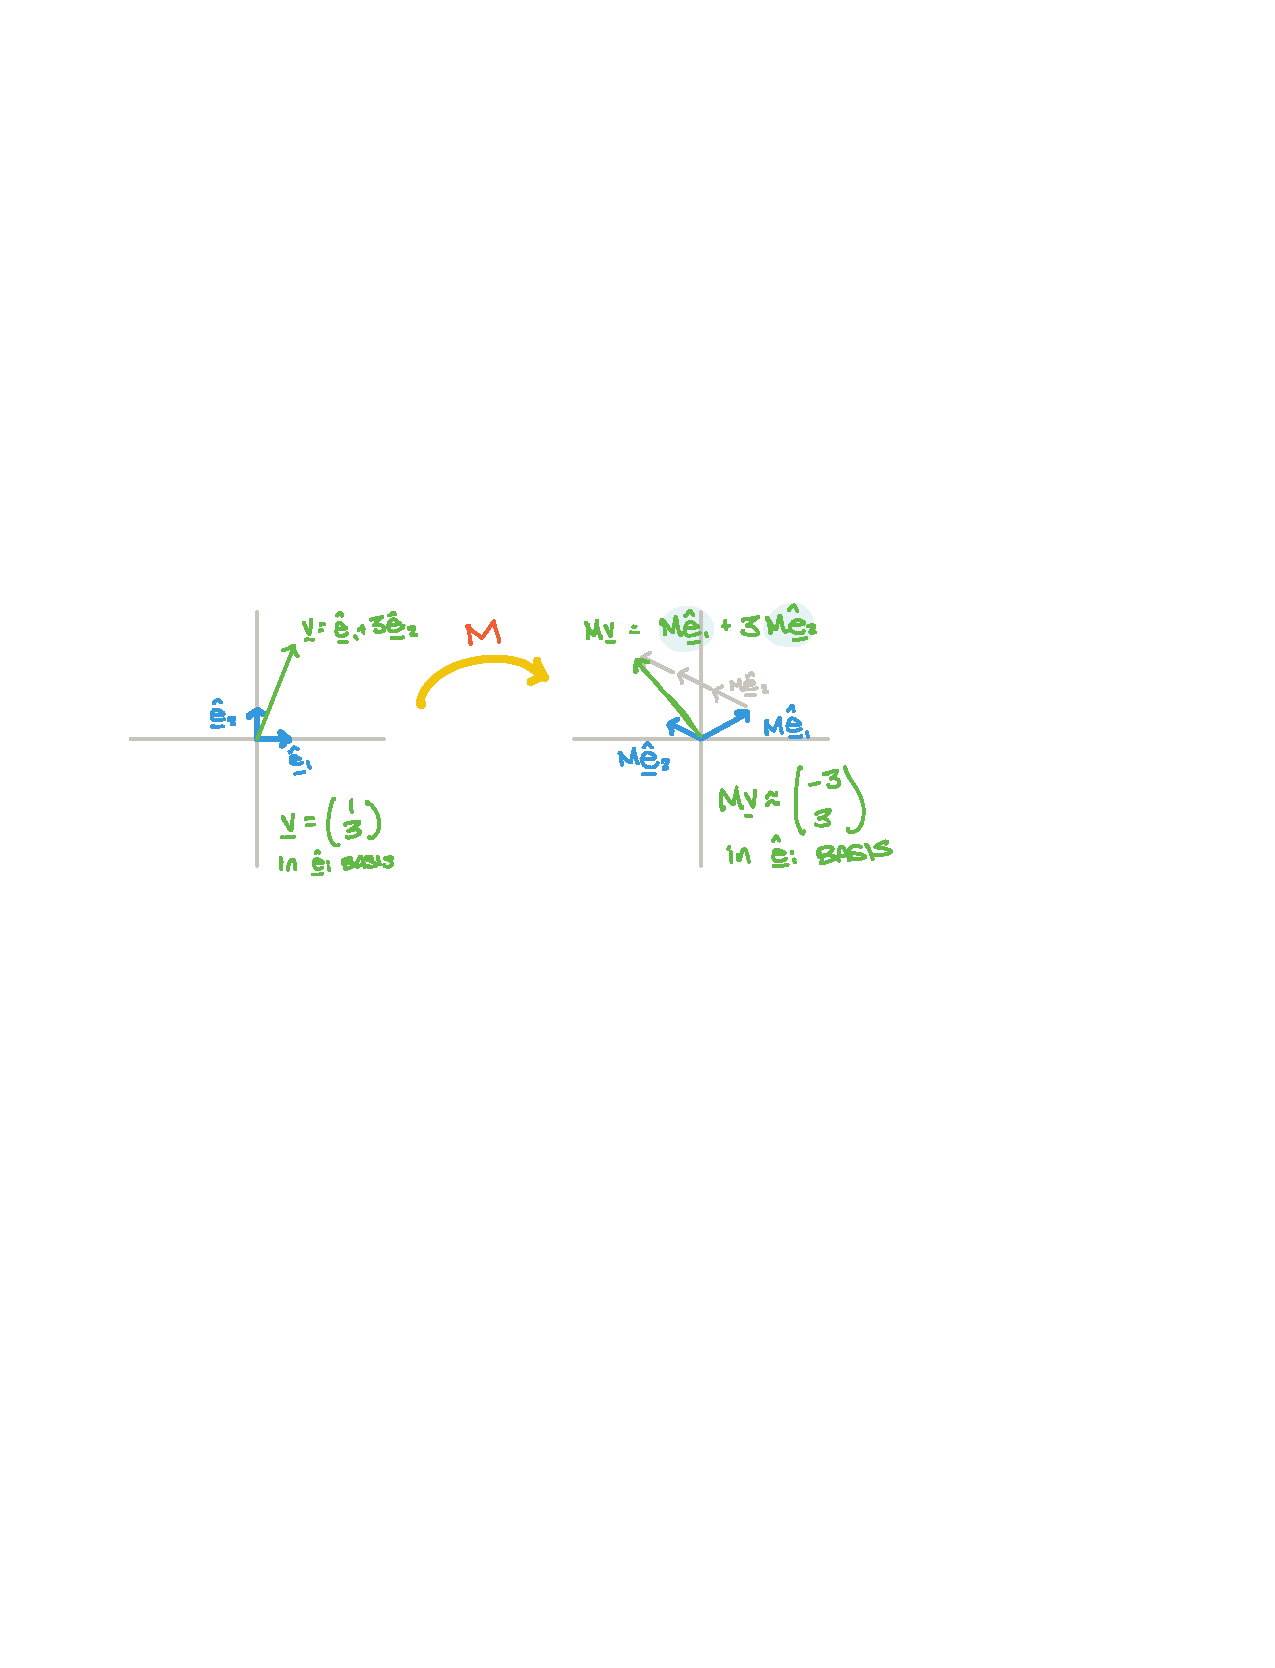
\includegraphics[width=.8\textwidth]{figures/maps_M.pdf}
%     \caption{.}
%     \label{fig:}
% \end{figure}

%% THEOREM ENVIRONMENTS


%% Because mdframed causes a bunch of warnings
%% https://tex.stackexchange.com/questions/64331/disable-warning-from-mdframed 
\usepackage{silence}
\WarningFilter{mdframed}{You got a bad break}
\WarningFilter{mdframed}{correct box splittet fails}



\newmdtheoremenv[
    skipabove=2em,
    skipbelow=2em,
    linewidth=5pt,
    linecolor=red!50!black,
    topline=false,
    rightline=false,
    bottomline=false
    ]{exercise}{Exercise}[section]


\newmdtheoremenv[
    skipabove=2em,
    skipbelow=2em,
    linewidth=5pt,
    linecolor=gray,
    topline=false,
    rightline=false,
    bottomline=false
    ]{example}{Example}[section]

\newmdtheoremenv[
    skipabove=2em,
    skipbelow=2em,
    linewidth=5pt,
    linecolor=blue,
    topline=false,
    rightline=false,
    bottomline=false
    ]{bigidea}{Key Idea}[section]

%% AMS Theorem version
% \newtheorem{exercise}{Exercise}[section]
% \newtheorem{example}{Example}[section]

%% Example: replace YourName with your name
\newcommand{\YourName}[1]{{	
	\color{blue!50!black}\footnotesize
	[\textbf{\textsf{YourName}}: \textsf{#1}]}}


\renewcommand{\tilde}{\widetilde}   % tilde over characters
\renewcommand{\vec}[1]{\mathbf{#1}} % vectors are boldface
\newcommand{\bas}[1]{\hat{\mathbf{#1}}} 	% basis vectors have hat
\newcommand{\row}[1]{\tilde{\mathbf{#1}}} 	% row vectors have tilde

% For matrices
\newcommand{\aij}[2]{^{#1}_{\phantom{#1}#2}}
\newcommand{\mat}[3]{#1\aij{#2}{#3}}
\newcommand{\pp}{\phantom{+}}
\newcommand{\inv}{^{-1}}


\usepackage{pifont}
	\newcommand{\cmark}{\ding{51}}%
	\newcommand{\xmark}{\ding{55}}%


%% COMMANDS FOR TEMPORARY COMMENTS
%% -------------------------------
\newcommand{\comment}[2]{\textcolor{red}{[\textbf{#1} #2]}}
\newcommand{\flip}[1]{{
	\color{green!50!black}
  \footnotesize
  [\textbf{\textsf{Flip}}: \textsf{#1}]
	}}

\newcommand{\correction}[2]{{
	\color{green!50!black}
  \footnotesize
  [\textbf{\textsf{Correction,~#1}}: \textsf{#2}]
	}}
